% !Mode:: "TeX:UTF-8" 

\chapter{\hei \textbf{研究背景}}

%=========================================================================================
\section{\hei 逻辑回归问题}

   	考虑逻辑回归问题
$$
\min _{x} \frac{1}{m} \sum_{i=1}^{m} \log \left(1+\exp \left(-b_{i} a_{i}^{T} x\right)\right)+\mu\|x\|_{2}^{2},
$$
其中 $\left(a_{i}, b_{i}\right)_{i=1}^{m}$ 为已知的待分类的数据集。 $\mu=1 e-2 / m$. 求解该优化问题。 该优化问题目标函数的梯度和海瑟矩阵:

$$
\begin{aligned}
	\nabla f(x) &=\frac{1}{m} \sum_{i=1}^{m} \frac{1}{1+\exp \left(-b_{i} a_{i}^{T} x\right)} \cdot \exp \left(-b_{i} a_{i}^{T} x\right) \cdot\left(-b_{i} a_{i}\right)+2 \mu x, \\
	H(x) &=\frac{1}{m} \sum_{i=1}^{m} \frac{\exp \left(-b_{i} a_{i}^{\top} x\right)}{\left(1+\exp \left(-b_{i} a_{i}^{\top} x\right)\right)^{2}} a_{i} a_{i}^{\top}+2 \mu I .
\end{aligned}
$$

我们可以使用矩阵语言将以上结果用更紧凑的形式表达. 引入矩阵 $A=\left[a_{1}, a_{2}, \cdots, a_{m}\right]^{T} \in R^{m \times n}$, 向量 $b=\left(b_{1}, b_{2}, \cdots, b_{m}\right)^{T}$.

{\hei 实际上,此逻辑回归问题可以简化为最优化问题当中的无约束优化问题。}


\section{\hei 无约束优化}
\subsection{最优化问题}

最优化是人们在工程技术、交通运输、经济金融和国防等诸多领域经常遇到的问题。例如,资源分配要使各用户利用有限资源产生的效益最大化;建筑设计要在满足设计需求的条件下所需预算尽可能少等等。总体而言,最优化问题就是人们为了达到预想目标,同时使各项生产经济活动中的人力、物力、财力的花费尽可能的少,在诸多预选方案中研究并选择出相对最优的一个或是多个方案的问题。

最优化问题解决实际方案通常由两个步骤组成:一是把需要求解的问题表述成数学上最优化问题的形式;二是在已有模型基础上选择已有的优化方法或者自己设计某种方法对模型进行求解\cite{杨庆之2015最优化方法}。

而在本次实验报告中我们主要关注最优化问题当中的无约束优化问题。

 \subsubsection{无约束优化问题}

作为优化领域的重要分支和约束优化领域的基础部分,无约束优化问题的核心问题在于寻求高效的数值求解方法。其对自变量$ x $的取值范围不施加任何约束条件,因此无需考虑$ x $的可行性,且很多无约束优化问题的思想可以较好的推广到其他的优化问题上去。

随着大型计算机和工作站的出现,诸多高效的最优化算法也随之出现与发展,并在未知变量规模较大的问题上取得了较好的效果。

无约束优化问题主要研究:
\begin{equation}\label{min}
	\min f(x) ,x \in \mathbb{R}^{n}
\end{equation}
的最优性条件,它包括一阶条件和二阶条件。
其中$ f: \mathbb{R}^{n} \rightarrow \mathbb{R} $称为目标函数,$ x $是变量。设$ x_{k} $为当前迭代点,$ g_{k}=\nabla f(x_{k}), G_{k}=\nabla^{2}f(x_{k})$分别表示函数$ f $在$ x_{k} $点处的梯度与Hessian矩阵。

无约束优化问题的极小点类型主要有局部较小点和全局极小点两种。全局极小点一定是局部极小点,反之不然,一般来说,求解全局极小点相当困难,因此我们通常把求解局部极小点作为实际应用当中的需求。
\begin{figure}[t]
	\centering
	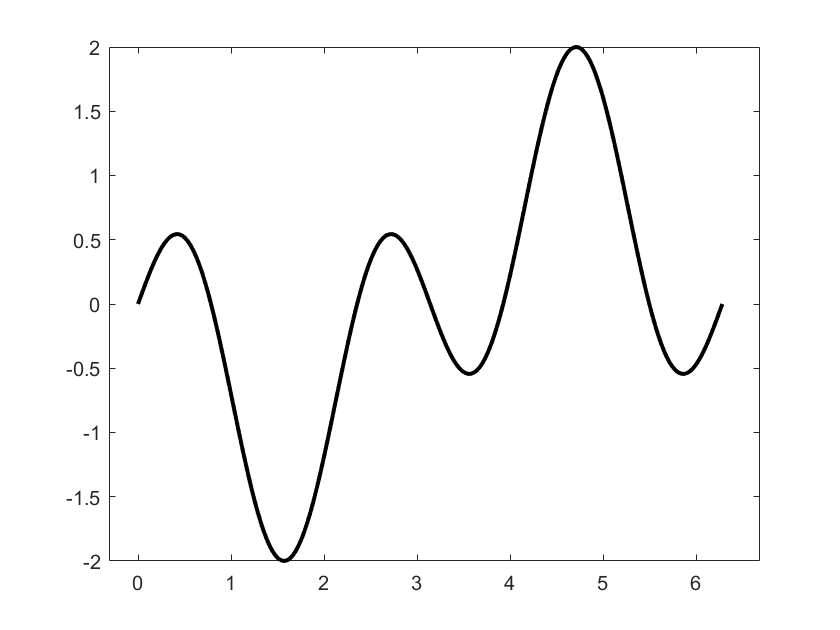
\includegraphics[scale=0.4]{figures/极小值.png}
	\caption{求解全局优化的一个例子}
\end{figure}

\subsection{无约束优化问题的基本算法}

在数值优化中,一般采取迭代法求解无约束优化问题的极小点。
迭代法的基本思想是:给定一个初始点$ x_{0} $,按照某一迭代规则产生一个迭代序列$ \{ x_{k}\}$。使得若该序列是有限的,则最后一个点就是问题\ref{min}的极小点;否则,若$ \{ x_{k}\} $是无穷点列时,它有极限点且这个极限点即为问题\ref{min}的极小点。

无约束优化算法问题的优化算法主要分为两大类:线搜索类型的优化算法和信赖域类型的的优化算法。他们都是对函数$ f(x) $在局部进行近似,但处理近似问题的方式不同。线搜索类算法根据搜索方向的不同可以分为梯度类算法、次梯度算法、牛顿算法、拟牛顿算法等.一旦确定了搜索的方向,下一步即沿着该方向寻找下一个迭代点.而信赖域算法主要针对 $ f(x) $ 二阶可微的情形,它是在一个给定的区域内使用二阶模型近似原问题,通过不断直接求解该二阶模型从而找到最优值点\cite{刘浩洋2021最优化}

在本次报告中,我们则主要关心线搜索类算法中的梯度类算法。

\section{\hei 梯度类算法}
\subsection{线搜索类算法}

我们首先需关心线搜索类算法,其数学表述为:给定当前的迭代点$ x_{k} $,首先通过某种算法选取向量$ d_{k} $,之后确定正数$ \alpha_{k} $,则下一步的迭代点可写作
\begin{equation}
	x_{k+1}=x_{k}+\alpha_{k}d_{k}
\end{equation}
我们称$ d_{k} $为迭代点$x_{k}  $处的搜索方向,$  \alpha_{k}$为相应的步长。这里要求$ d_{k} $是一个下降方向,即$ (d_{k})^{T} \nabla f(x_{k}) <0$。这个下降性质保证了沿着此方向搜索函数$ f $的值会减小。线搜索类算法的关键是如何选取一个好的方向$ d_{k} \in \mathbb{R}^{n} $以及合适的步长$  \alpha_{k}$。

下面,我们给出求解无约束优化问题\ref{min}的线搜索类算法一般框架如下:

\begin{algorithm}[H]	
	\floatname{algorithm}{算法}
	\caption{(一般下降算法)}
	\renewcommand{\algorithmicrequire}{\textbf{输入:}} 
	\renewcommand{\algorithmicensure}{\textbf{输出:}}
	
	\begin{algorithmic}[1]
		\State  给定初始点$ x_{0} \in \mathbb{R}^{n} $,令$ k:=0 $
		\State  计算$ g_{k}=\nabla f(x_{k}) $,若$ \| g_{k} \| \leq \epsilon$,停算,输出近似极小点$ x^{*} \approx x_{k} $
		\State  依照一定规则,\textbf{确定下降方向$ d_{k} $.}
		\State  \textbf{计算步长因子$ \alpha_{k} $},使其满足某个下降规则
		\State  置$ x_{k+1} = x_{k}+\alpha_{k}d_{k}, k:=k+1 $,转步骤2.
	\end{algorithmic}
\end{algorithm}	

\subsection{梯度类算法}

梯度类算法(Gradient Method)以负梯度作为搜索方向,成为所有需计算导数的优化算法中最简单的方法,也是最优化中最基本的算法。梯度类算法所需内存少,对于求解大规模问题较为适用。

梯度法中步长的选取至关重要,最古老也是最经典的\textbf{最速下降法}(Steepest Descent Method),源自1847年的Cauchy\cite{cauchy1847methode},迭代过程中每次都需经过线搜索求得步长因子,但是在实际问题当中,最速下降方向仅是算法的局部性质,并非“最速下降”,而是下降非常缓慢。数值实验证明,当目标函数的等值线是一个扁长的圆球时,最速下降法开始几步下降较快,后来就出现锯齿现象,下降十分缓慢\cite{akaike1959successive,forsythe1968asymptotic}。

一些最新的研究\cite{de2013spectral,nocedal2002behavior}还证明了其具有的一些新的性质。

Barzilai和Borwein\cite{barzilai1988two}于1988年对梯度类算法提出的改进\textbf{两点步长梯度法}(Barzilai-Borwein Gradient Method),因其对于梯度类算法计算效率的极大改善,再度引发了学界关于梯度法的研究热潮,对其进行了大量效果优异的改进,这也是本次实验报告所关注的内容。

\subsection{最大似然估计}
最大似然估计是一种统计方法,它用来求一个样本集的相关概率密度函数的参数。这个方法最早是遗传学家以及统计学家罗纳德·费雪爵士在1912年至1922年间开始使用的。
“似然”是对likelihood 的一种较为贴近文言文的翻译,“似然”用现代的中文来说即“可能性”。故而,若称之为“最大可能性估计”则更加通俗易懂。

{\hanyi 最大似然法明确地使用概率模型,其目标是寻找能够以较高概率产生观察数据的系统发生树。最大似然法是一类完全基于统计的系统发生树重建方法的代表。该方法在每组序列比对中考虑了每个核苷酸替换的概率。}
例如,转换出现的概率大约是颠换的三倍。在一个三条序列的比对中,如果发现其中有一列为一个C,一个T和一个G,我们有理由认为,C和T所在的序列之间的关系很有可能更接近。由于被研究序列的共同祖先序列是未知的,概率的计算变得复杂;又由于可能在一个位点或多个位点发生多次替换,并且不是所有的位点都是相互独立,概率计算的复杂度进一步加大。尽管如此,还是能用客观标准来计算每个位点的概率,计算表示序列关系的每棵可能的树的概率。然后,根据定义,概率总和最大的那棵树最有可能是反映真实情况的系统发生树。

\begin{table}
	\renewcommand{\arraystretch}{1.2}
	\centering\wuhao
	\caption{表题也是五号字} \label{tab_ch2} \vspace{2mm}
	\begin{tabular}{c@
			{\hspace{1cm}}c@{\hspace{1cm}}c@{\hspace{1cm}}c}
		\toprule[1.2pt]
		Interference & DOA (deg) & Bandwidth (MHz) & INR (dB) \\
		\midrule[0.8pt]
		1 & $-30$ & 20 & 60 \\
		2 & 20 & 10 & 50 \\
		3 & 40 & 5 & 40 \\
		\bottomrule[1.2pt]
	\end{tabular}
\end{table}

\begin{example}
	随机变量$Z_i = (X_i, Y_i), i=1, 2,\cdots, n$ 属于独立同分布. $X_i,Y_i$有两个可能的取值0或者1. 
	$P(X_i=1)=\alpha, P(Y_i=1|X_i)=\beta X_i$ (一般地,$X_i$与$Y_i$不是相互独立).
	$n$是一个正整数,$0<\alpha<1$, $0<\beta<1$是未知参数,请解答下面的问题:
\begin{itemize}
	\item[(1)] 确定$P(X_i, Y_i)$在$(x,y)$取所有可能的值的分布律,可用$\alpha$和$\beta$表示;
	\item[(2)] $Z_i, i=1, 2,\cdots, n$, 利用所有$Z_i$去估计$\alpha$和$\beta$的最优估计$\hat{\alpha}_n$和 $\hat {\beta}_n$;
	\item[(3)] 假设$\alpha + \beta=1$, 求在该约束条件下,利用$Z_i$计算$\alpha$的最优估计量$\hat{\alpha}_n$;
	\item[(4)] 在第(3)问中,当$n\to\infty$,$\hat{\alpha}_n$收敛于一个值,求该值.
\end{itemize}
\end{example}


解:(1) $Z_i=(X_i,Y_i)$的分布律为
\begin{center}
	\begin{tabular}{|c|c|c|c|c|}
		\hline
		$(X_i,Y_i)$	& $(0,0)$ & $(0,1)$ & $(1,0)$ & $(1,1)$\\
		\hline
		$p_k$	& $1-\alpha$ & $0$ & $\alpha(1-\beta)$ & $\alpha\beta$\\
		\hline
	\end{tabular}
\end{center}


(2) 把以上分布律写成一个通式
\begin{subequations}
	\begin{align}
		P\{X_i=x\}&=\alpha^{x}(1-\alpha)^{1-x},\\
		P\{Y_i=y|X_i=x\}&=(\beta x)^{y}(1-\beta x)^{1-y}, \label{aa}\\
		P\{X_i=x,Y_i=y\}&=\alpha^{x}(1-\alpha)^{1-x}(\beta x)^{y}(1-\beta x)^{1-y}.\label{bb}
	\end{align}
\end{subequations}
如果将式子\eqref{aa}、\eqref{bb}中$0^0$定义为1, 那么通式\eqref{bb}和联布律表格的意思相同.
但是$0^0$在教材上是没有意义的,可恶的$0^0$!

\begin{center}
\textcolor{blue}{\hei
不要慌,不要慌,太阳落下有月光;\\
不要慌,不要慌,抄手吃完还有汤.}
\end{center}

当$x=0,y=0$时, 底数$\beta x$增加一个量$1-x-y$, 这样底数就不是$0$, 也就不会产生$0^0$.
于是\eqref{aa}、\eqref{bb}可改写为
\begin{subequations}
	\begin{align}
		P\{Y_i=y|X_i=x\}&=[(\beta-1)x+1-y]^{y}(1-\beta x)^{1-y}, \tag{\ref{aa}'} \label{aa'}\\
		P\{X_i=x,Y_i=y\}&=\alpha^{x}(1-\alpha)^{1-x}[(\beta-1)x+1-y]^{y}(1-\beta x)^{1-y}.\tag{\ref{bb}'}  \label{bb'}
	\end{align}
\end{subequations}
至此, 通式\eqref{bb'}和分布律表格的意思完全相同.

于是,似然函数为
\begin{align}
L(\alpha,\beta)
&=\prod_{i=1}^n P\{X_i=x_i,Y_i=y_i\} \notag\\
&=\prod_{i=1}^n \alpha^{x_i}(1-\alpha)^{1-x_i}[(\beta-1)x_i+1-y_i]^{y_i}(1-\beta x_i)^{1-y_i} \notag\\
&= \alpha^{\sum\limits_{i=1}^n x_i}(1-\alpha)^{n-\sum\limits_{i=1}^n x_i}\beta^{\sum\limits_{i=1}^n x_iy_i}(1-\beta)^{\sum\limits_{i=1}^n x_i(1-y_i)} \label{cc}
\end{align}
%
注意上式中$\sum\limits_{i=1}^n x_iy_i$表示$n$个样本取值中$(1,1)$的个数;
$\sum\limits_{i=1}^n x_i(1-y_i)$表示$n$个样本取值中$(1,0)$的个数.

为了求$L(\alpha,\beta)$的最大值点, 先对\eqref{cc}两边取对数, 得
$$
\ln L(\alpha,\beta)=
{\sum\limits_{i=1}^n x_i}\ln\alpha
+(n-\sum\limits_{i=1}^n x_i)\ln(1-\alpha)
+{\sum\limits_{i=1}^n x_iy_i}\ln\beta
+{\sum\limits_{i=1}^n x_i(1-y_i)}\ln(1-\beta).
$$
可求得最大值点, 即最大似然估计值为
$$
\hat{\alpha}_n=\frac{1}{n}\sum\limits_{i=1}^n x_i,\quad
\hat{\beta}_n=\frac{\sum\limits_{i=1}^n x_iy_i}{\sum\limits_{i=1}^n x_i}.
$$

(3)
当$\beta=1-\alpha$时, 似然函数$L(\alpha,\beta)$可改写为
$$
\ln L(\alpha,1-\alpha)=
(2\sum\limits_{i=1}^n x_i-\sum\limits_{i=1}^n x_iy_i)\ln\alpha
+(n-\sum\limits_{i=1}^n x_i+\sum\limits_{i=1}^n x_iy_i)\ln(1-\alpha).
$$
此时, $\alpha$的最大似然估计值为
$$
\hat{\alpha}_n=\frac{2\sum\limits_{i=1}^n x_i-\sum\limits_{i=1}^n x_iy_i}{n+\sum\limits_{i=1}^n x_i}.
$$

(4) 注意到,当$n\to \infty$时, $\dfrac{1}{n}\sum\limits_{i=1}^n x_i\to P\{X=1\}=\alpha$,
$\dfrac{1}{n}\sum\limits_{i=1}^n x_iy_i\to P\{X=1,Y=1\}=\alpha(1-\alpha)$ (频率趋于概率).
因此
$$
\lim_{n\to\infty}\hat{\alpha}_n=\frac{2\alpha-\alpha(1-\alpha)}{1+\alpha}=\alpha.
$$



